\chapter{CUDA}

This chapter describes the Compute Unified Device Architecture, better known by its acronym CUDA, a "general purpose parallel computing platform and programming model" \citep{site:cuda}, which allows simplified utilization of NVIDIA Graphics processing units (GPU) for solving complex computational problems.

First we describe the advantages and disadvantages of the GPU hardware. Next we describe the basic programming model, after which we provide more detail about features useful for parallelization of cross-correlation.

\section{GPU}
\label{sec:gpu}

Central processing unit (CPU) is optimized to process a single stream of instructions working on a single stream of data as fast as possible. This requires CPU design to minimize instruction latency, which is achieved by using branch predictions, multiple levels of caching, and other such mechanisms. On the other hand, GPU is optimized for throughput of a single stream of instructions working on many streams of data. The single stream of instructions is executed many times in parallel, which allows GPU to hide high latency operations by switching to other threads instead of trying to optimize for lower latency of each instruction. The thread switching is made instantaneous by keeping the execution context, such as registers, of all threads resident at all times.

This leads to the principle of \textbf{occupancy}, where GPU requires high number of threads to properly hide the high latency of each operation. Especially for small inputs, care needs to be taken so that the processing is split between enough threads to saturate the GPU.

The need to assign each thread separate registers in the register file as part of the execution context also highlights one of the limiting factors of occupancy, \textbf{register pressure}. Code requiring too many registers may limit the number of threads which can actually be executed in parallel, limiting occupancy, or leading to register spilling into slower types of memory, limiting performance.


\section{Programming model}
\label{sec:programming_model}

CUDA distinguishes two parts of the system running two types of code. First is the \textit{host} code running on the host part of the system. This is standard C++ program running on the CPU, accessing system memory and calling the operating system, as any other standard C++ program would. The second part is the \textit{device} code, running on a device or on multiple devices. Each device corresponds to a single GPU \footnote{Since Compute Capability 8.0 Ampere, device can represent a GPU slice.}.

Both parts of the code are programmed in the same language, CUDA C++, which is an extension to the C++ language, with some restrictions to the device code and some parts of the language only usable in the device code.
One of the important things CUDA C++ introduces are \textit{function execution space specifiers}, which are attributes added to a function declaration and which specify if the given function is part of the host code, device code or if it should be compiled both for host and device code. The available \textit{function execution space specifiers} are:
\begin{itemize}
	\item \texttt{\_\_global\_\_}, which declares the function as being a kernel, callable from host code and executed on the device,
	\item \texttt{\_\_device\_\_}, which declares the function as executed on the device, callable by another device or global function,
	\item \texttt{\_\_host\_\_}, which declares the function as executed on the host, callable from the host only.
\end{itemize}

Without any specifiers, function is compiled as part of the host code. \textbf{Kernel} is a function with the \texttt{\_\_global\_\_} specifier, which is callable from the host code but is executed on a device. Kernels serve as entry points which the host code uses to offload computation to the device. Kernel invocation is asynchronous, where the function call to the kernel in host code does not wait for the kernel on the device to finish but returns immediately after the kernel is submitted.

When invoking a kernel, host code specifies the number of threads which are to run the device code. The abstraction defining the behavior of the device code, called the SIMT execution model, is described in the subsection \ref{sec:simt}.

\subsection{Single Instruction, Multiple Threads}
\label{sec:simt}

The device code, written in CUDA C++ as a part of \textit{global} or \textit{device} function, describes the behavior of a single thread running on the device. Compared to host code running on the CPU, the device code is always ran by many threads simultaneously.



In the Single instruction, multiple threads(SIMT) execution model, threads on the device are split into groups of 32, called \textit{warps}. Each warp of threads is scheduled together, starting at the same program address and executing in lockstep.\footnote{Since Compute Capability 7.0 Volta, threads of a warp can be scheduled more independently and do not execute strictly in lockstep \citep{paper:volta}.}
If branching occurs, as can be seen in Figure \ref{fig:thread_divergence_old}, any branch that is taken by at least a single thread of a warp is executed by the whole warp, masking out any threads that did not take given branch. When masked, thread does not execute any reads or writes, but still has to continue execution with other threads in the warp. This is most apparent in loops, where a single thread of a warp executing the loop thousand times will result in the whole warp executing the loop thousand times, even if other threads are masked and do nothing for most of the loops. This cuts the theoretical throughput by a factor of 32, as only one of the 32 threads does useful work.

\begin{figure}[ht]
	\centering
	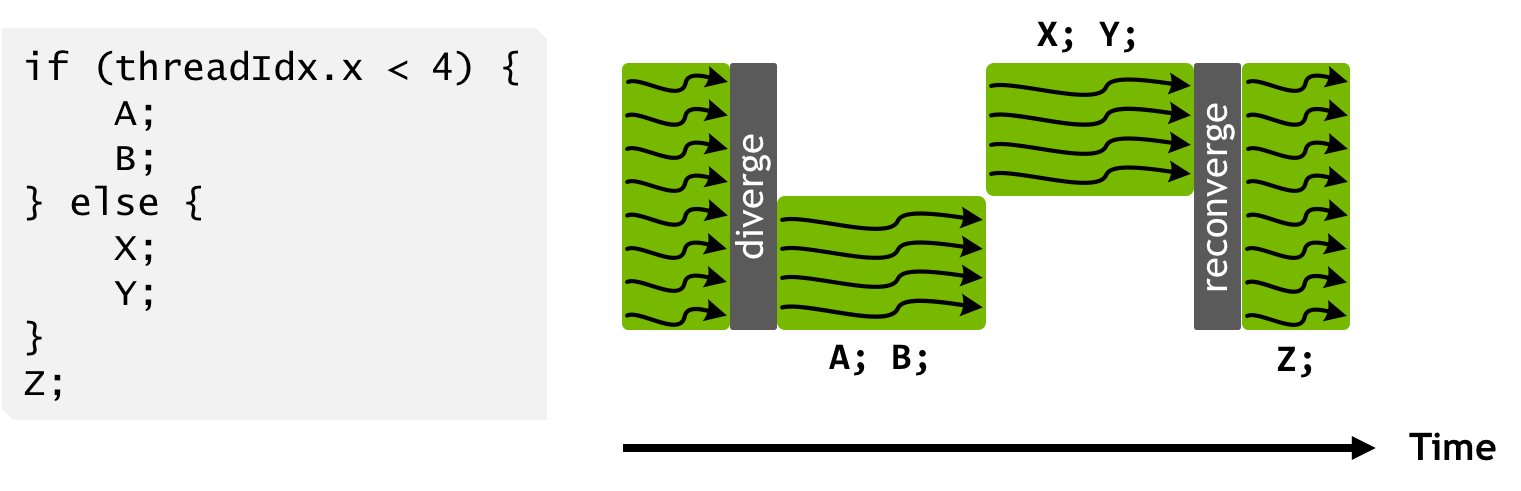
\includegraphics[width=0.8\textwidth]{cuda_thread_divergence_old.png}
	\caption{Branching in device \citep{site:cuda}.}
	\label{fig:thread_divergence_old}
\end{figure}

% TODO: Maybe mention global memory access

On the surface, the device code is very similar to the host code written for the CPU, and will most likely work correctly if written as if for the CPU. But to maximize performance, one must keep in mind the SIMT model, grouping into warps, thread divergence when branching, coalesced memory accesses etc.

On the other side of the spectrum, the SIMT execution model can be compared to the Single instruction, multiple data (SIMD) execution model, where the number of elements processed by a single instruction is directly exposed in the user code, compared to the SIMT model, where the user code itself describes a behavior of a single thread and the grouping of threads is abstracted by the platform. 

\subsection{Thread hierarchy}
\label{sec:thread_hierarchy}

Apart from being grouped into warps, threads on the device are also grouped into Cooperative Thread Arrays (CTA), also known as thread blocks. Thread blocks can be one-dimensional, two-dimensional or three-dimensional, which provides an easy way to distribute work when processing arrays, matrices or volumes. Thread blocks are further organized into one-dimensional, two-dimensional or three-dimensional grid, as can be seen in Figure \ref{fig:thread_hierarchy}. When launching a kernel, we specify thread block size and grid size, which combined together give us the number of threads executing the given kernel.

\begin{figure}[ht]
	\centering
	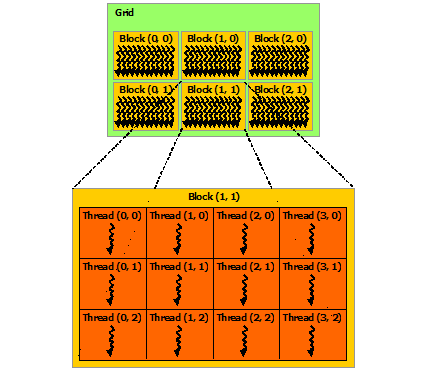
\includegraphics[width=0.8\textwidth]{grid_of_thread_blocks.png}
	\caption{Thread grouping hierarchy \citep{site:cuda}.}
	\label{fig:thread_hierarchy}
\end{figure}

Each thread is assigned an index, accessible through \texttt{threadIdx} built-in variable. Each thread can also access the index of the thread block it is part of through \texttt{blockIdx}, the block size through \texttt{blockDim} and grid size through \texttt{gridDim}. All of these variables are three dimensional vectors, with dimensions unused during kernel launch set to zero for indices and one for dimensions. Using these built-in variables, we can distribute work between threads, most often assigning each thread a part of the input to process.

\subsection{Thread cooperation}
\label{sec:thread_cooperation}
CUDA provides several mechanisms for thread cooperation. Threads can cooperate on the following levels of thread hierarchy, with increasing speed and capability:

\begin{itemize}
	\item grid level,
	\item thread block level,
	\item warp level.
\end{itemize}

The rest of this subsection describes the older API using intrinsic functions. The newer Cooperative Groups API, which is a superset of the older API, is described in Subsection \ref{sec:cooperative_groups}.

\subsubsection{Grid level}
On grid level, the only available tools for cooperation are atomic operations on global memory. These operations can be used to perform read-modify-write on a 32-bit or 64-bit word in global memory without introducing race conditions.

\subsubsection{Thread block level}
On a thread block level, threads can use two mechanisms for cooperation:
\begin{itemize}
	\item shared memory,
	\item synchronization barrier.
\end{itemize}

As per the CUDA C++ programming guide: 
"the shared memory is expected to be a low-latency memory near each processor core (much like an L1 cache) and \_\_syncthreads() is expected to be lightweight" \citep{site:cuda}.

Shared memory is a small on-chip memory, described in more detail in the subsection \ref{sec:memory_hierarchy}. Each thread block has private shared memory, accessible only from threads of the given thread block. Shared memory can be used as software managed cache or to share results between threads of the thread block. 

To synchronize access to shared memory between threads of the thread block, we use synchronization barrier \texttt{\_\_syncthreads()}. All threads in the block must execute the call to \texttt{\_\_syncthreads()} before any of the threads can proceed beyond the call to \texttt{\_\_syncthreads()}. 
The \texttt{\_\_syncthreads()} function also serves as memory barrier. % TODO: Maybe describe what memory barrier is

\subsubsection{Warp level}
% TODO: Describe masks for all the functions
On warp level, threads of the warp, or lanes as they are referred to in the documentation, can utilize intrinsic functions to exchange data without the use of shared memory and perform simple hardware accelerated operations. For operations, warps can perform:
\begin{itemize}
	\item reduce-and-broadcast operations,
	\item broadcast-and-compare operations,
	\item reduce operations,
\end{itemize}

% This is important as this is the basis of one of our algorithms
For data exchange, CUDA C++ provides several warp shuffle instructions. There are four source-lane addressing modes:
\begin{itemize}
	\item direct lane index,
	\item copy from lane with ID lower by \textit{delta},
	\item copy from lane with ID higher by \textit{delta},
	\item copy from lane based on bitwise XOR of provided \textit{laneMask} and own lane ID. 
\end{itemize}

The data exchange does not have to span the whole warp. Shuffle operations allow the warp to be subdivided into groups with width of a power of 2.

Only direct lane indexing performs lane index wrap around. If the given lane index is out of the range $[0:width - 1]$, the actual lane index is computed as: $srcLane \mod width$. In other addressing modes, the lanes with out of range source lane index are left unchanged, receiving the value they pass in. The wrap around mechanism allows us to rotate data between threads instead of just shifting. The direct lane indexing can also be used to broadcast a value from a single lane to all other lanes. % TODO: Maybe mention how the wrap around can be used to implement ring buffer shifting between two parts of a buffer

For warp level operations, the reduce-and-broadcast operations receive a single integer value from each lane which they compare to zero, making it effectively a boolean. The results of the comparison are then reduced in one of the following ways and the result is broadcast to all threads:
\begin{itemize}
	\item result is non-zero if and only if all of the values are non-zero,
	\item result is non-zero if any of the values are non-zero,
	\item result contains single bit for each lane which is set if the value given by the lane was non-zero
\end{itemize}

The broadcast-and-compare operations broadcast the value given by each lane and compare it to the value given by the current lane, returning:
\begin{itemize}
	\item mask of lanes that have the same value,
	\item mask if all threads in mask gave the same value, 0 otherwise.
\end{itemize}

Finally, there are the general reduce operations. \textit{Add}, \textit{min}, \textit{max} operations are implemented for signed or unsigned integer values. \textit{And}, \textit{or}, \textit{xor} operations are implemented for unsigned integers only.

The API described in this subsection forms the basis of thread cooperation in CUDA. Most of this API is available since the early versions of CUDA. Subsection \ref{sec:cooperative_groups} will describe the newer Cooperative groups API, which builds on top of and extends the API described in this subsection.

\subsection{Cooperative groups}
\label{sec:cooperative_groups}

Cooperative Groups API, introduced with CUDA 9, is an extension to the CUDA programming model for organizing groups of communicating threads \citep{site:cuda}. The API introduces data types representing groups of cooperating threads, be it a warp, a part of a warp, a thread block, a grid or even a multigrid\footnote{Multigrid represents multiple grids each running on a separate device.}.


The API distinguishes two types of groups. First are the \textit{implicit groups}, which are present implicitly in each CUDA kernel. These are:

\begin{itemize}
	\item thread block,
	\item grid,
	\item multigrid.
\end{itemize}

The API provides functions to create handles to objects of data types representing the implicit groups. 

The other type are \textit{explicit groups}, which must be explicitly created from one of the implicit groups. 

\begin{itemize}
	\item thread block tile,
	\item coalesced group.
\end{itemize}

Both of these groups represent warp or subwarp size grouping of threads. Thread block tile can be created from a thread block or from another thread block tile, representing a warp or a part of a warp of size of a power of 2. The warp level operations described in the previous subsection \ref{sec:thread_cooperation} are available as methods on this group, with mask and width arguments of the built-in functions implicitly derived from the properties of the group. 

% TODO: Explaing coalesced group


Creating a handle for an implicit group is a collective operation, in which all threads of the group must participate. Creating the group handle in a conditional branch may lead to deadlocks or data corruption. It may also introduce unnecessary synchronization points, limiting concurrency. Similarly to implicit group handle creation, partitioning of groups is a collective operation which must be executed by all threads of the parent group and may introduce synchronization points. It is recommended to create implicit group handles and do all partitioning at the start of the kernel and pass const references throughout the code \cite{site:cuda}.

\subsection{Memory hierarchy}
\label{sec:memory_hierarchy}

Each CUDA device has its own DRAM memory, so called \textit{device memory} or \textit{VRAM}, which is separate from the host system memory and from the \textit{device memory} of all other devices. Physically, \textit{device memory} can be seen on most GPU boards as DRAM chips separate from the main silicon chip.

Data transferred between the host and device memory has to be transferred over the PCI-e bus, either explicitly by calls to \textit{cudaMemcpy} in the host code or by mapping parts of host memory to the \textit{device memory} address space using the \textit{Unified Memory} system, which then handles the data transfers in the background automatically.

From the point of view of a CUDA thread, there are several types of memory available, as can be seen in Figure \ref{fig:memory_types}. For this thesis, the main types are:

\begin{itemize}
	\item local memory,
	\item shared memory,
	\item global memory,
	\item registers.
\end{itemize}

\begin{figure}[ht]
	\centering
	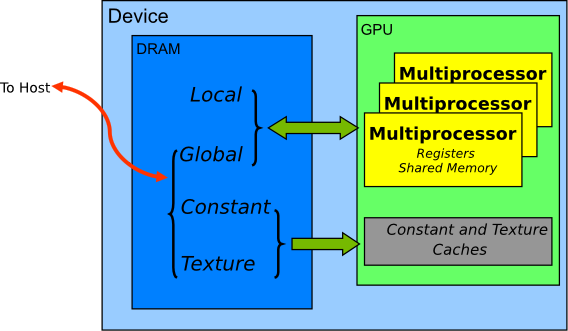
\includegraphics[width=0.8\textwidth]{memory-spaces-on-cuda-device.png}
	\caption{Memory types on a CUDA device \citep{site:cuda}.}
	\label{fig:memory_types}
\end{figure}

Local and global memory are both allocated from device memory, and as such have very high access latency. 

\textbf{Local memory} is private for each thread, allocated automatically based on the requirements of the CUDA compiler. This type of memory is used for register spilling, arrays with non-constant indexing and large structures or arrays which would consume too much register space. 

\textbf{Global memory} is shared by all threads of a kernel, and as such any access which could lead to race condition must be synchronized using atomic operations, as described in Section \ref{sec:thread_cooperation}. Global memory is allocated by the host code using \texttt{cudaMalloc} family of functions. When host code transfers data to the device using \texttt{cudaMemcpy} or any other means, global memory is the part of device memory this data will be transferred to. The pointers returned by \texttt{cudaMalloc} and possibly used in \texttt{cudaMemcpy} are then passed as arguments to the kernel. Device code can then use these to access the global memory. 

\textbf{Shared memory}, as mentioned in the section \ref{sec:thread_cooperation}, is expected to be a low-latency memory near each processor core (much like an L1 cache). The relation with L1 cache can be seen in the fact that each kernel can configure the proportion between hardware allocated to L1 cache and to Shared memory, which means these memories share the same underlying hardware. Shared memory can be allocated either dynamically by declaring an array type variable with the memory space specifier \texttt{\_\_shared\_\_} and providing the size to be allocated during kernel launch, or statically by defining the variable with static size.


\textbf{Registers} are the fastest memory available for device code. Compared to CPUs, GPUs provide large amount of registers. For all recent GPU generations, the register file provides 65536 32bit registers. 

\subsection{Streaming multiprocessor}
\label{sec:sm}
NVIDIA GPUs are build around an array of \textit{Streaming multiprocessors} (SM). SM of a GPU is similar to a core of a multicore CPU. Each SM has separate execution units, schedulers, register file, shared memory and L1 cache. An example of an SM can be seen in Figure \ref{fig:volta_sm}. Each SM can have multiple schedulers, each scheduling up to one warp per cycle. 

Each thread block is assigned to a single SM exclusively, and each SM can run multiple thread blocks at once. Warps of all thread blocks resident on the given SM are scheduled regardless of the thread block the warps belong to.

% TODO: More

\begin{figure}[ht]
	\centering
	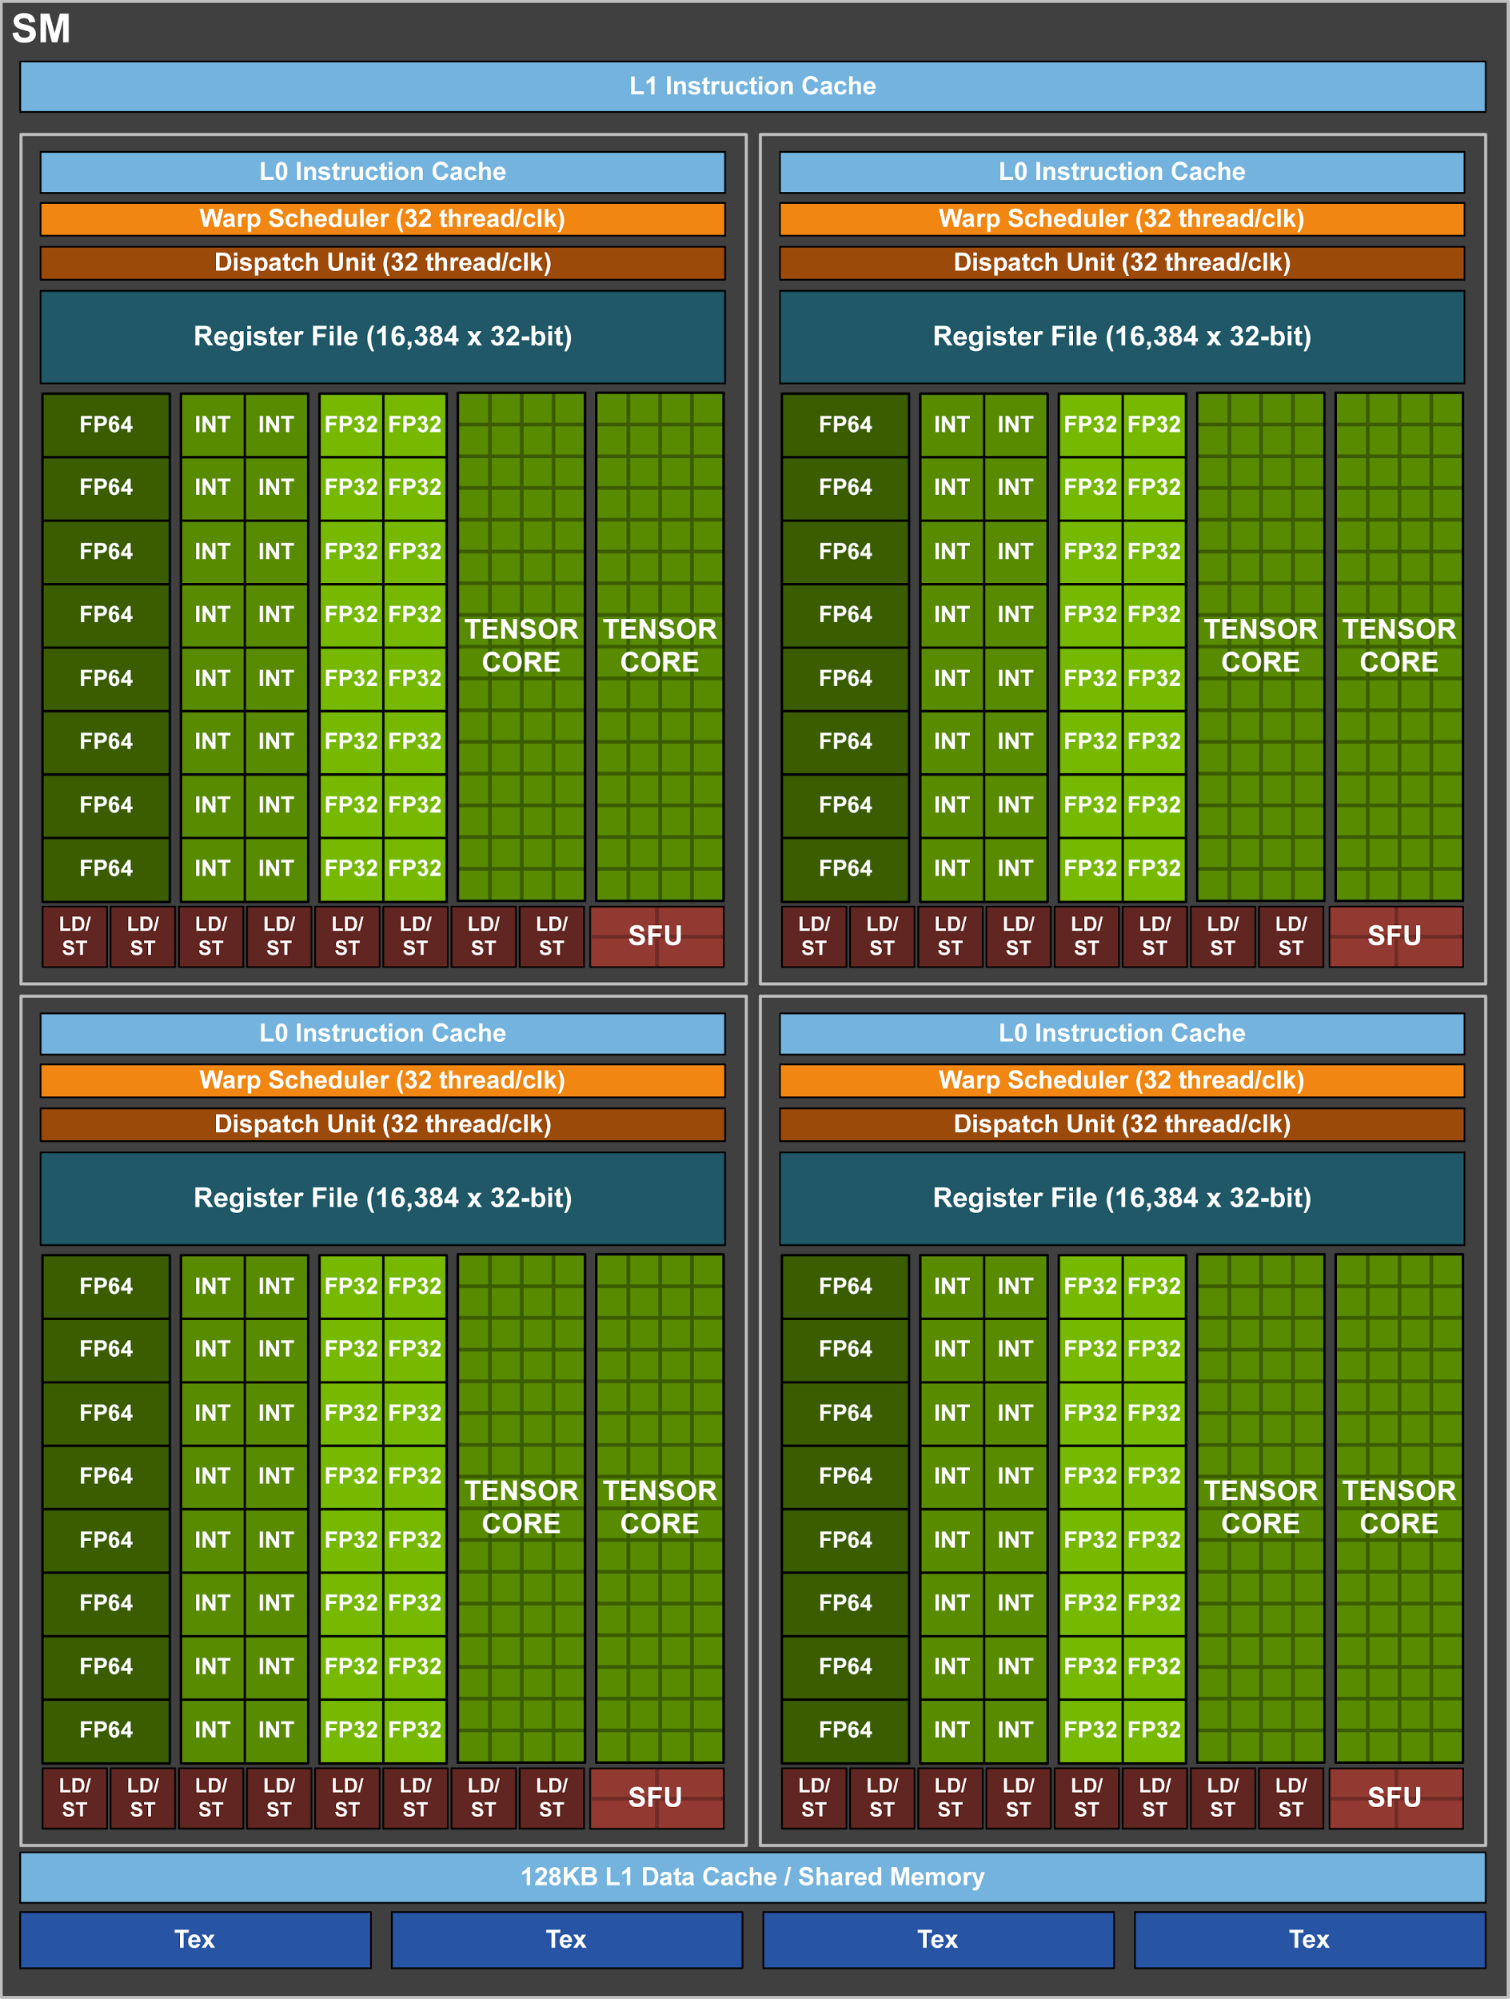
\includegraphics[width=0.8\textwidth]{volta_sm.png}
	\caption{Streaming multiprocessor \citep{paper:volta}.}
	\label{fig:volta_sm}
\end{figure}

\subsection{Versioning}

When working with CUDA, there are two main parts of the platform which are versioned separately: % TODO: Add driver version
\begin{itemize}
	\item CUDA Toolkit,
	\item GPU Compute Capability.
\end{itemize}

CUDA Toolkit represents the software development part of the CUDA platform, encompassing the CUDA runtime library, the \textit{nvcc} compiler and other tools for development of the software.

GPU Compute Capability (CC) represents the features provided by the hardware. This includes the number of registers, memory sizes, set of instructions etc. In general, each consumer GPU generation corresponds to a new CC, such as GTX 1000 cards corresponding to CC 6.0 Pascal and RTX 3000 cards corresponding to CC 8.0 Ampere. There are some exceptions, for example CC 7.0 Volta having only enterprise cards. With each release of new Compute Capability cards, there is generally accompanying CUDA Toolkit release providing access to the new features provided by the hardware. 

Compute Capabilities are backwards compatible, so code created for older generation of cards can be ran on newer cards, even though it may not take advantage of new hardware features and may be inefficient on the newer cards.

\section{Code optimizations}


This section introduces basic principles for producing performant CUDA code.
The observations and recommendations provided in this section are based on the principles and properties described in the previous section \ref{sec:programming_model}.

\subsection{Occupancy}
\label{sec:occupancy}

The GPU design prioritizes high instruction throughput of many concurrent threads over single thread performance at the cost of high latency of each instruction. To hide the high latency between dependent instructions, each scheduler keeps a pool of warps between which it switches, possibly on each instruction. Warps in a pool of a scheduler are called \textit{active} warps.
Each cycle, there may be multiple warps which have instructions ready to be executed. Such warps are called \textit{eligible} warps.
Each cycle, a warp scheduler can select one of the \textit{eligible} warps as \textit{issued} warp, issuing its instruction to be executed.

For optimal performance, we want to have enough active warps so that there is at least one eligible warp each cycle to enable the GPU to hide the high latency of each instruction. As described in Section \ref{sec:sm}, the number of warps resident on a SM depends on the number and size of thread blocks resident on a SM.

The number of thread blocks assigned to an SM is limited by three factors:

\begin{itemize}
	\item hardware limit,
	\item register usage,
	\item shared memory usage.
\end{itemize}

The hardware limit differs, but is either 16 or 32 for all currently supported Compute Capabilities. 

To enable no cost execution context switching (program counters, registers, etc.), the whole execution context for all warps is kept on the SM for the whole lifetime of each warp. 


Number of registers used by all warps of all blocks which reside on the given SM must be smaller than or equal to the number of registers in the register file. For example, for SM with 65536 registers, code using 64 registers per thread and 512 threads in a block, there can only be two blocks resident on the SM, as $2*512*64 = 65536$. If the code requires just a single register more, only a single block will be resident on each SM.

The total amount of shared memory required by all blocks residing on an SM must be smaller than or equal to the size of shared memory provided by the SM. 

\subsection{Pipeline saturation}
\label{sec:cuda_pipelines}

Other than occupancy, there are other possible reasons why no warp may be eligible in a given cycle. Pipeline saturation is one of such reasons. GPU hardware has several pipelines, each implementing a different part of the instruction set. As an example, for the RTX 2060 card, these include:
\begin{itemize}
	\item Load Store Unit (LSU),
	\item Arithmetic Logic Unit (ALU),
	\item Fused Multiply Add/Accumulate (FMA),
	\item Transcendental and Data Type Conversion Unit (XU).
\end{itemize}

Each instruction has a Compute Capability specific throughput, which if exceeded, makes the pipeline implementing the instruction saturated and unable to execute any other instructions. This becomes a problem when, for example, many or all warps often execute the same low throughput instruction, such as sinus, cosinus or inverse square root, which are implemented by the XU pipeline. Even for simpler operations implemented by the ALU or FMA, if all warps execute the same instruction, the pipelines may become saturated and warps which are waiting to execute more of the given instruction will not be eligible to be issued.

High LSU utilization reflects that the program may be memory bound, waiting for data from global or shared memory, or that the program executes many warp shuffle instructions, which are also implemented by the LSU pipeline. Due to this, the usage of shared memory together with warp shuffles is not advisable, as they both utilize the same pipeline and compete for resources.

% TODO: Maybe screenshot from NSIGHT Compute

\subsection{Global memory access}

As shown in Figure \ref{fig:global_memory_access}, each access to global memory is grouped into 128~B naturally aligned chunks, where any chunk accessed by any of the threads of a warp has to be transferred from global memory. The maximum performance is achieved when access to memory is aligned and coalesced, i.e. all threads of a warp access elements in the same 128~B chunk which is aligned to 128~B. Any other form of access introduces overhead in a form of unnecessary data being transferred from global memory. 

When accessing data larger than 32 bits, the access is split into 2 half-warp transactions for 64 bit or 4 quarter warp transactions for 128 bit values, which are then processed independently, again reading any 128~B chunk any of the accesses. 

Access to global memory goes through at least one level of cache. On older architectures, global memory accesses are by default only cached in L2 cache, with L1 cache utilized only for local memory access to speed up register spills. % TODO: referece https://docs.nvidia.com/cuda/cuda-c-programming-guide/index.html#compute-capability-3-0
Special instructions can be used to cache data in L1 explicitly. For Compute Capabilities newer than 5.0, compiler can generate an instruction to load read-only data, such as the two input matrices in cross-correlation, and cache it in L1 cache. L1 cache, with cache line size of 128~B, is local to each SM and shares hardware with shared memory, described in the following section. L2 cache, with cache line size of 32~B, is still on-chip but is shared by all SMs. Each 128~B memory transfer is either served by a single L1 cache access or split into 4 32~B L2 cache accesses.

\begin{figure}[ht]
	\centering
	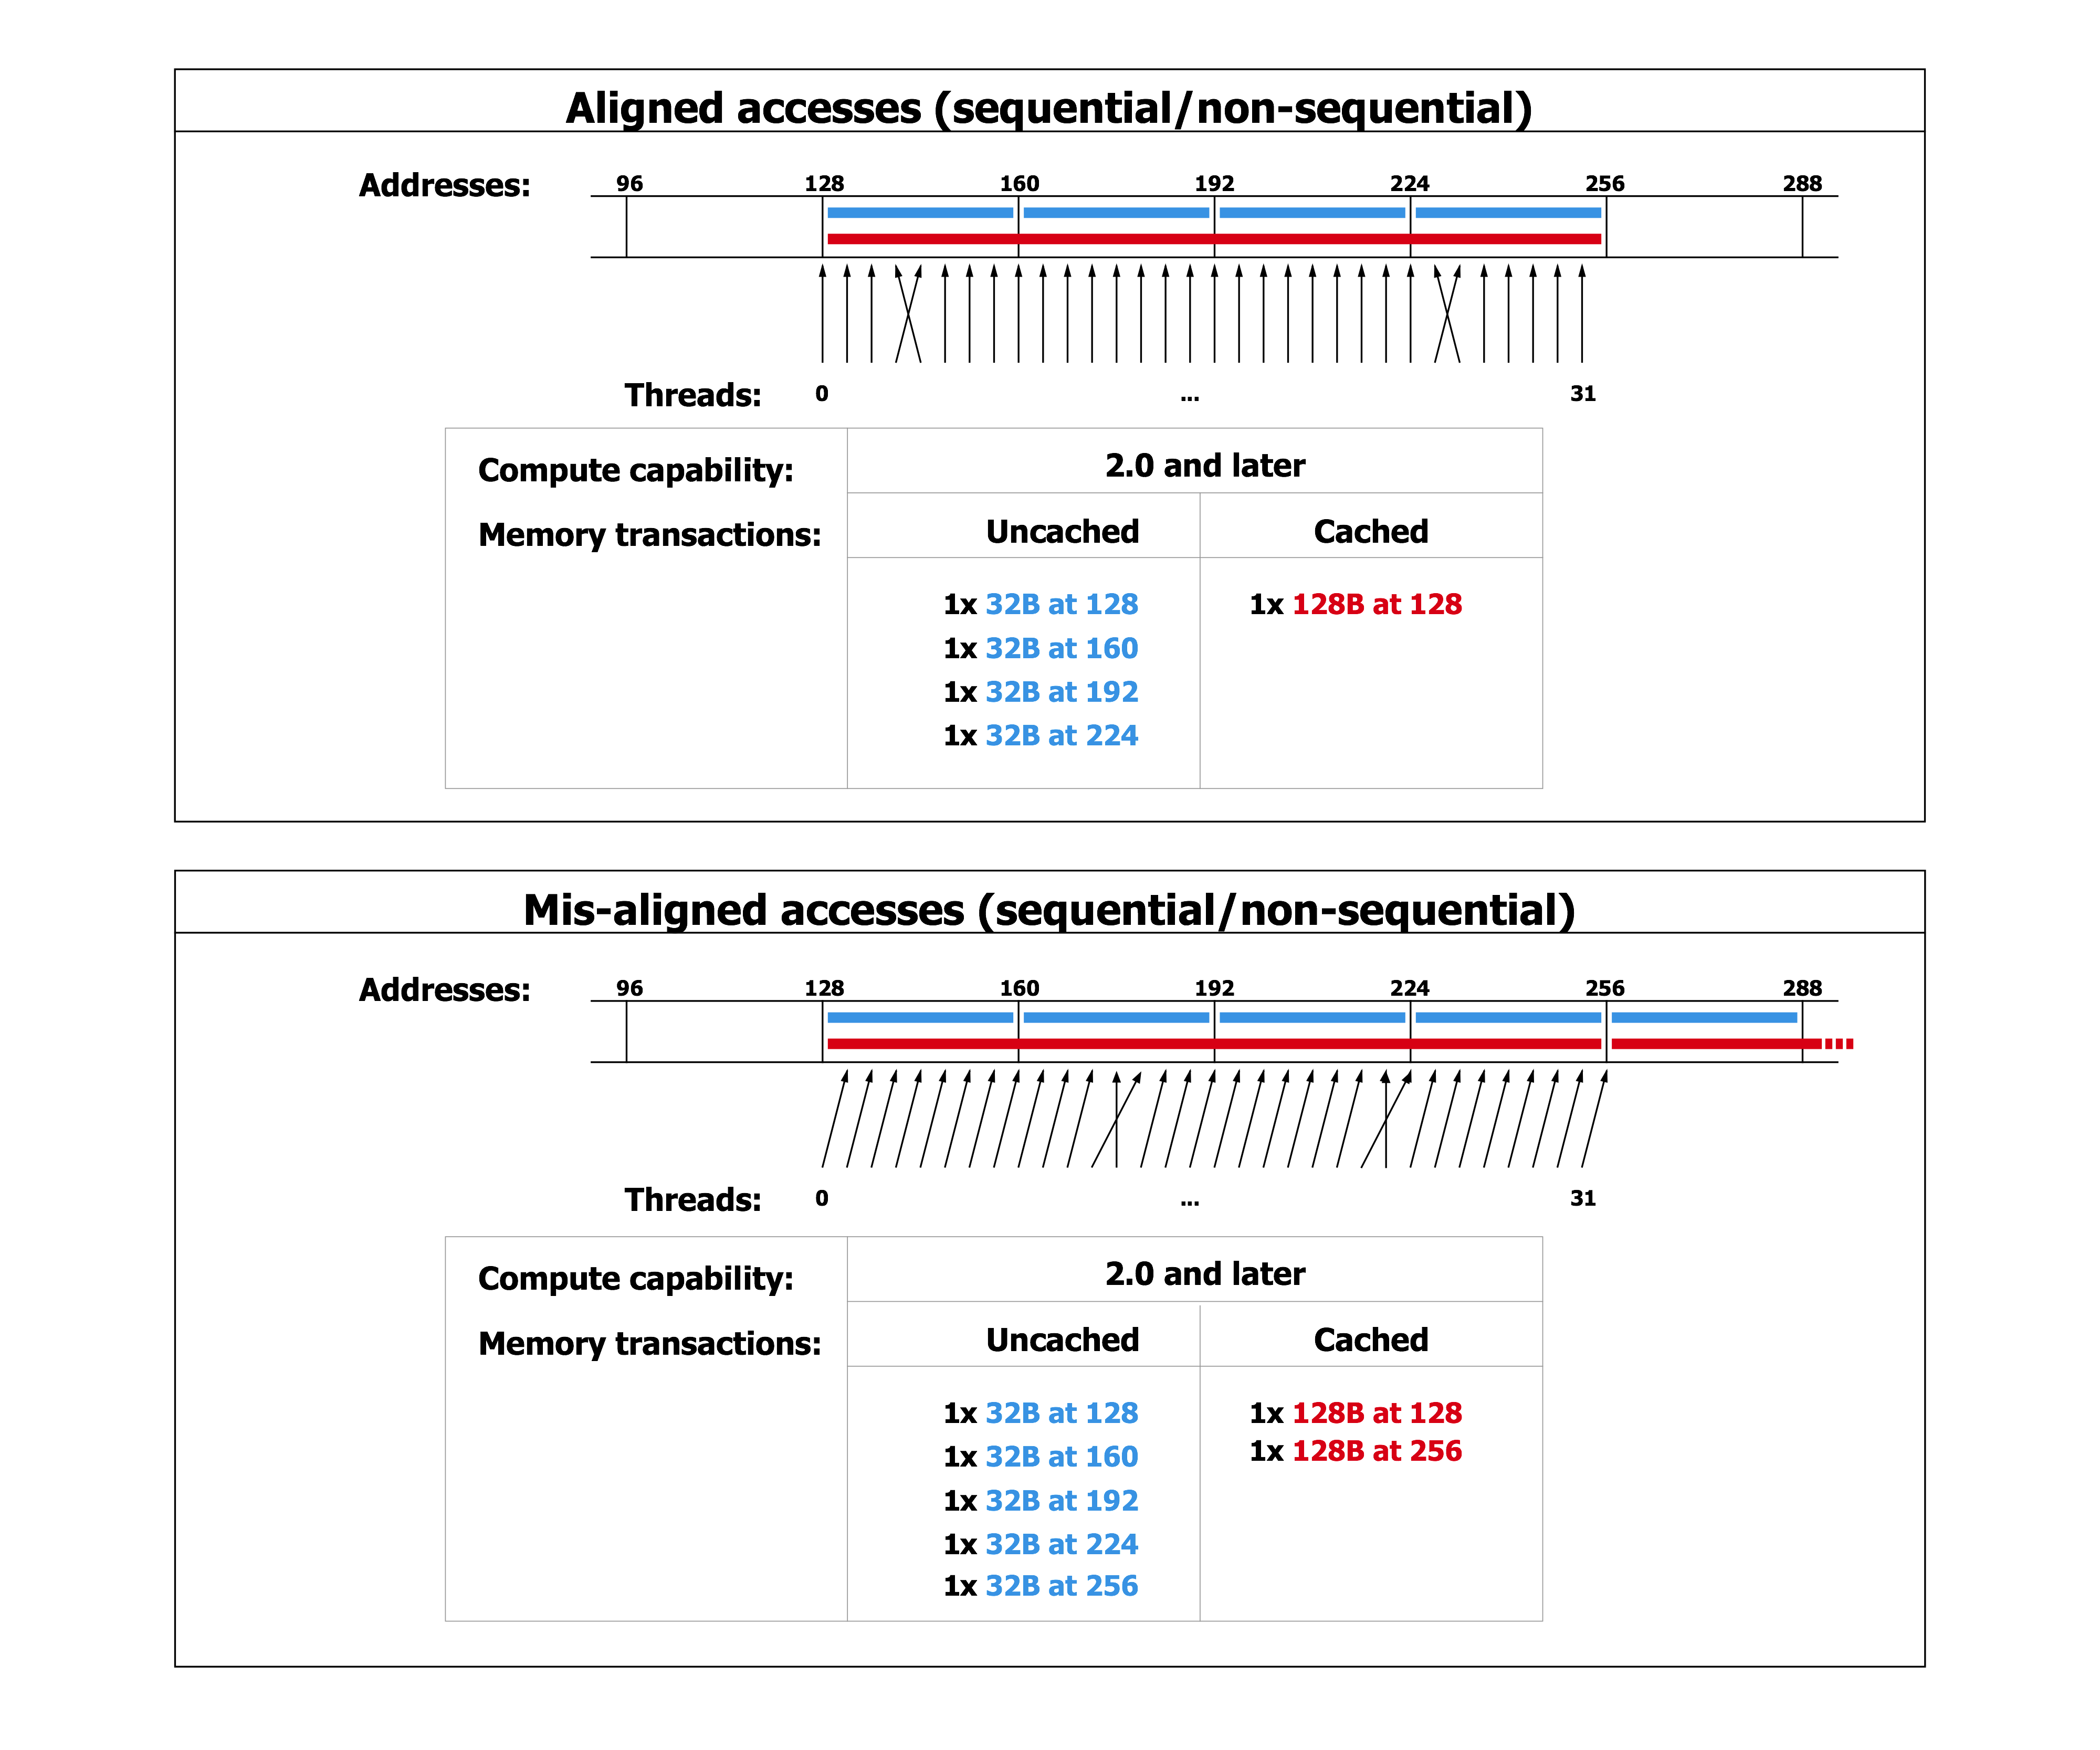
\includegraphics[width=0.8\textwidth]{global-memory-access.png}
	\caption{Global memory access \citep{site:cuda}.}
	\label{fig:global_memory_access}
\end{figure}

\subsection{Shared memory access}
To achieve high bandwidth, shared memory is divided into 32 banks. The optimal access pattern the shared memory is designed for is for each thread of a warp to access a different bank. To enable this access pattern, successive 32bit words are mapped to successive shared memory banks. The simplest pattern is that the 32 threads of a warp access 32 consecutive 32bit items from an array in shared memory, as can be see in the left column of Figure \ref{fig:shared_memory_access}. If multiple threads access different addresses mapping to the same bank, as can be seen in the middle column of the figure, their accesses are serialized, the throughput of shared memory being divided by the maximum number of different addresses accessed in any of the banks. This is called a \textit{bank conflict}. Access to the same address by multiple threads does not lead to a bank conflict, instead leading to a broadcast of the value between the threads.

\begin{figure}[ht]
	\centering
	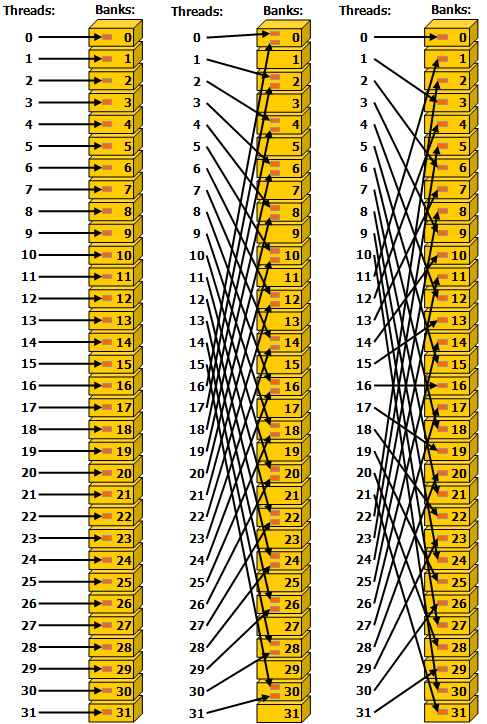
\includegraphics[width=0.8\textwidth]{shared-memory-access.png}
	\caption{Shared memory access patterns \citep{site:cuda}.}
	\label{fig:shared_memory_access}
\end{figure}

\subsection{General recommendations}

We can summarize the information in previous subsections into few simple rules \citep{site:cuda}:

\begin{enumerate}
	\item Maximize parallel execution to achieve maximum utilization;
	\item Optimize memory usage to achieve maximum memory throughput;
	\item Optimize instruction usage to achieve maximum instruction throughput.
\end{enumerate}

To maximize parallel execution, ensure that the workload is distributed between large enough number of threads, where each thread requires low enough number of registers and each thread block requires small enough part of shared memory so that enough thread blocks fit onto an SM.

To optimize memory usage, minimize transfers from lower bandwidth memory by reusing data in hardware cache or manually move data to shared memory. When accessing global memory, utilize coalesced accesses to minimize unnecessary data transferred. When accessing shared memory, minimize bank conflicts.

To optimize instruction usage, minimize the use of low throughput instructions such as sinus, cosinus or inverse square root. When working with floating point numbers, use 32 bit numbers if precision is not crucial. Minimize thread divergence to ensure all threads in a warp execute useful instructions.

% TODO: Move related work to Analysis chapter
%\section{Related work}

% Accelerating Radio Astronomy Cross-Correlation with Graphics Processing Units

% Kapinchev GPU Implementation of Cross-Correlation for Image Generation in Real Time





